\documentclass[12pt, a4paper]{scrartcl}

% --packages--
\usepackage[utf8]{inputenc}
\usepackage[italian]{babel}
\usepackage{graphicx}
\usepackage{mathtools}
\usepackage{MnSymbol}
\usepackage{fancyvrb}
\usepackage{hyperref}
\setlength{\parindent}{0pt}
\def \a {\textsf{A}}

\subtitle{\textbf{Università degli studi di Milano-Bicocca}}
\subtitle{\textbf{Data warehouse}}
\title{\textbf{Analisi della correlazione tra incidenti e tempo atmosferico a New York}}
\subtitle{\textbf{Periodo temporale: 2015-2017}}

\author{Danilo Deponti - 737838 $    $ Mattia Curatitoli - 735722} \date{}


\begin{document}
\maketitle
 
\section*{Introduzione}
introduzione

\section*{Analisi dei dati - Csv Incidenti}

\subsection*{Sorgente dati: Incidenti a New York}
Il dataset contenente gli incidenti stradali avvenuti a New York nel periodo temporale da noi analizzato è stato ottenuto attraverso la piattaforma \emph{NYC Open Data} nella sezione \emph{Sicurezza pubblica}.
Il sito mette a disposizione numerosi sistemi per filtrare i dati sugli incidenti stradali, come quello per lasso temporale, utilizzato nel progetto. E' possibile esportare questi dati in formato \emph{CSV, TSV, XML, RSS e RDF}
\subsection*{Informazioni raccolte}
Analizzando il massiccio dataset ricavato, sono state rilevate le seguenti informazioni che lo caratterizzano:
\subsubsection*{Incidente}
L'incidente è l' entità caratterizzante del dataset, questa entità fornisce informazioni come la chiave univoca dell' incidente, data, ora, posizione (latitudine, longitudine) e numero di morti/feriti coinvolti.
Sia per i morti che per i feriti è possibile sapere se erano pedoni, ciclisti o conducenti.
Inoltre, vi sono anche informazioni riguardanti il tipo di veicolo e in quale modo il relativo veicolo può avere provocato l' incidente.
\subsubsection*{Anagarafica Tipologia veicolo}
Analizzando attentamente il dataset è stato riscontrato che la descrizione della tipologia del veicolo è identica e si ripete per moltissimi incidenti. Su circa 700000 incidenti analizzati sono state rilevate solamente 200 tipologie di veicolo distinte, tra le quali più della metà sono comprensibili. Molto probabilmente, per la maggior parte degli incidenti è stato compilato un form di reportistica dove la tipologia di veicolo era definita tra un elenco. 
\subsubsection*{Anagrafica Scatenante}
Come già illustrato nel precedente paragrafo, anche per lo scatenante è possibile distinguere un numero finito e molto ridotto (circa 60) di dati che caratterizzano quasi costantemente gli incidenti. Addirittura, per questa informazione, il numero di scatenanti rilevate che non hanno significato è ridotto allo 0.

\subsection*{Schema logico relazionale}
I dati recuperati sono stati forniti in un unico e decisamente ricco csv. I dati, per ogni incidente, erano riportati su una sola riga e non vi era alcuna logica di riutilizzo dei dati. Inoltre, appunto per come sono stati archiviati i dati, non vi era alcuna logica di normalizzazione.
E' stato quindi deciso di scomporre i dati ricavati nelle seguenti entità:
\newline
\newline
$incidente$ (\textbf{\underline{id}}, unique\_key,numero\_morti, numero\_feriti, pedoni\_morti, pedoni\_feriti, ciclisti\_morti, ciclisti\_feriti, conducenti\_morti, conducenti\_feriti, \textit{id\_luogo}, data\_incidente, ora\_incidente, created\_at, updated\_at)
\newline
La relazione $incidenti$ contiene tutte le informazioni che contraddistinguono l'incidente: data, ora, numero feriti, numero morti ed una distinzione di essi in pedoni, ciclisti e conducenti.
\newline
\newline
$scatenante$ (\textbf{\underline{id}}, descrizione)
\newline
Questa relazione contiene tutti i possibili motivi che hanno provocato l'incidente. Questa relazione, per mezzo del suo identificativo univoco intero, permette di associare il motivo scatenante all' incidente per mezzo di un' apposita tabella di collegamento.
\newline
\newline
$tipoVeicolo$ (\textbf{\underline{id}}, tipologia)
\newline
La relazione $tipoVeicolo$ definisce tutti i tipi di veicolo che possono caratterizzare l' incidente. Si collegano all' incidente, attraverso un identificativo univoco, per mezzo di un' apposita tabella di collegamento.
\newline
\newline
$dettagli$ (\textit{\underline{id\_incidente}},\textit{\underline{id\_tipoveicolo}},\textit{\underline{id\_scatenante}})
\newline
Questa relazione è ciò che collega l' incidente con i veicoli ed, eventualmente, in che modo il suddetto veicolo ha provocato l'incidente.
Il collegamento è creato tramite la tripletta di attributi $id_incidente$,$id_tipoveicolo$,$id_scatenante$.
Ogni incidente può avere molteplici righe di dettaglio. 
\newline
\newline
$luogo$ (\textbf{\underline{id}}, quartiere, zip, latitudine,longitudine)
\newline
La relazione luogo identifica
\newline
\newline
$strada$ (\textbf{\underline{id}}, strada)
\newline
\newline
$link\_luogo\_strada$ (\textit{\textbf{\underline{id\_luogo}}},\textit{\textbf{\underline{id\_strada}}})
\newline
\newline
\begin{center}

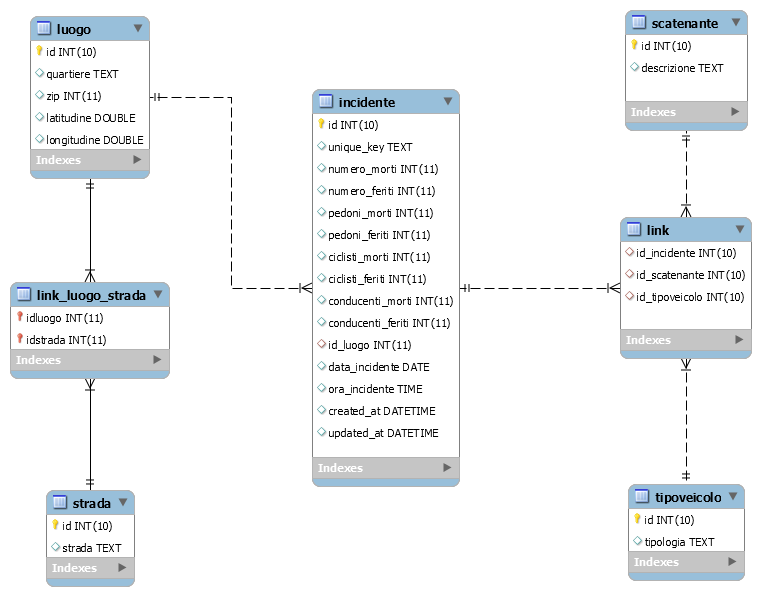
\includegraphics[scale=0.6]{ER.png}
\end{center}













\end{document}
